%---------------------------------------------------------------------
%
%                          Parte Proteopathogen
%
%---------------------------------------------------------------------
%

\addtocontents{toc}{\protect\bigskip}



\partTitle{
 %\begin{flushright}
  \sc{Desarrollo de una aplicaci�n web para recoger, visualizar y analizar resultados de estudios de prote�mica de \textit{Candida albicans}}
 %\end{flushright}
}


%~ \partDesc{ 
%~ \begin{FraseCelebre}
%~ \begin{Frase}
%~ An unmatched left parenthesis creates an unresolved tension \\
%~ that will stay with you all day
%~ \end{Frase}
%~ \begin{Fuente}
%~ Randall Munroe\\
%~ XKCD
%~ \end{Fuente}
%~ \end{FraseCelebre}
%~ }

%Sure, we seem like we've taken over the planet, but if I had to bet on
%which one of us would still be around in a million years primates, 
%computers, or ants, I know who I'd pick.

%My primary goal when designing Ruby was to have fun programming
%Yukihiro Matsumoto. 

\partDesc{ 

\hfill
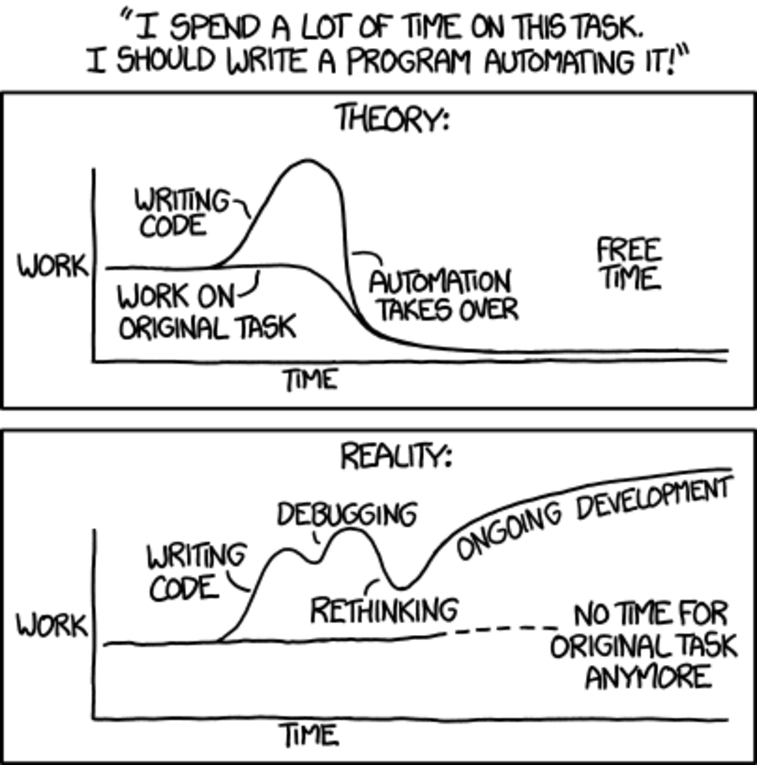
\includegraphics[width=0.7\textwidth]{Imagenes/Vectorial/automation}
\begin{FraseCelebre}
\begin{Fuente}
xkcd, Randall Munroe
\end{Fuente}
\end{FraseCelebre}

%\begin{FraseCelebre}
%\begin{Frase}
%Talk is cheap.\\
%Show me the code.
%Everybody stand back.\\
%I know regular expressions.
%My primary goal when designing Ruby was to have fun programming.
%Most good programmers do programming not because they expect to get paid or get adulation by the public, but because it is fun to program.
%\end{Frase}
%\begin{Fuente}
%Linus Torvalds.
%Yukihiro Matsumoto
%\end{Fuente}
%\end{FraseCelebre}

}

%\partBackText{}

%\makepart











\part%
[\sc{Desarrollo de una aplicaci�n web para recoger, visualizar \\%
y analizar resultados de estudios de prote�mica \\%
de \textit{Candida albicans}}]%
{\partTitleVal}\partDesc{}


\makeatletter
\renewcommand\part{%
  \if@openright
    \cleardoublepage
  \else
    \clearpage
  \fi
  \thispagestyle{empty}% Cambiado; antes era plain pero
% no queremos n�mero de p�gina...
  \if@twocolumn
    \onecolumn
    \@tempswatrue
  \else
    \@tempswafalse
  \fi
  \null\vspace*{2cm}% Cambiado; en vez de \vfil, un espacio fijo de
                    % dos cent�metros, para que el t�tulo no cambie de
                    % posici�n dependiendo de la longitud de la descripci�n.
  \secdef\@part\@spart}

% Versi�n "sin estrella" del comando part. Se mete en el toc y se pone
% "Parte I"; despu�s viene el t�tulo y descripci�n.
\def\@part[#1]#2{%
    \ifnum \c@secnumdepth >-2\relax
      \refstepcounter{part}%
      \addcontentsline{toc}{part}{\thepart\hspace{1em}#1}%
    \else
      \addcontentsline{toc}{part}{#1}%
    \fi
    \markboth{}{}%
    {\centering
     \interlinepenalty \@M
     \normalfont
     \ifnum \c@secnumdepth >-2\relax
       %\huge\bfseries \partname\nobreakspace\thepart %Esto es lo que escribe "Parte I"
       \par
       \vskip 20\p@
     \fi
     \huge \bfseries #2\par}
    % Si hay descripci�n de la parte, la ponemos despu�s de 2 cent�metros
    {\vspace*{2cm}\noindent\partDescVal}%
    \@endpart}



\def\@endpart{\vfil\newpage
              \if@twoside
               \if@openright
                \null
                \thispagestyle{empty}%
                {\partBackTextVal}
                \newpage
               \fi
              \fi
              \if@tempswa
                \twocolumn
              \fi}
\makeatother

